% for example, the time period of the backtest, the rebalancing frequency, the data resolution, transaction costs, etc.
    
To show the problems of Markowitz's minimum volatility portfolios in real applications, and compare these portfolios to the portfolios computed using other methods and techniques, each of the techniques described here is implemented for a portfolio of exchange traded products (ETPs) representing 4 assets classes: equities, fixed income, real estate and commodities. We use the QuantConnect platform \cite{qcwebsite} for the implementation and as the data source. This platform and its API allow us to perform backtests with one-minute resolution data. A backtest is nothing else than a simulation of a portfolio with past data to see how it would have behaved, if we had hold it during that past period considered in the backtest. With one-minute resolution data, we have price data that is sampled once per minute. This allows us to model the changes in portfolio value as well as the entry and closing price of orders accurately considering the fact that the holding period is at least one month.

\subsection{Selected ETPs}
    Due to the lack of Euro denominated ETP data in the QuantConnect data bank, we decided to use US dollar denominated ETPs which are intended for US based traders. For the selection of ETPs, we use iShares website \cite{isharesscreener}, because it provides a screener for its ETPs\footnote{Disclosure: the author of this thesis is not associated with iShares, BlackRock or any of its companies.}.
    
    For the equity ETPs, we selected equity index exchange traded funds (ETFs) with regional category "Global" by sectors and industries. From all of the ETPs fulfilling those conditions shown in the online screener, we chose the following ETFs (alphabetically ordered by ticker):
    % Equity alphabetically sorted.
    \begin{itemize}
        \item iShares Global Industrials ETF with ticker "EXI" which seeks to track the investment results of an index composed of global equities in the industrials sector. More specifically, the index tracked is the S{\&}P Global 1200 Industrials Sector Index (TM). The top sub-sectors represented in the ETF holdings are capital goods, transportation and commercial and professional services. Source: \href{https://www.ishares.com/us/literature/fact-sheet/exi-ishares-global-industrials-etf-fund-fact-sheet-en-us.pdf}{iShares Global Industrials ETF Fact Sheet as of June 30, 2021}.% \cite{factsheet_exi}.
    
        \item iShares MSCI Global Energy Producers ETF with ticker "FILL" which seeks to track the investment results of an index composed of global equities of companies primarily engaged in the business of energy exploration and production. More specifically, the index tracked is the MSCI ACWI Select Energy Producers Investable Market Index. The top sub-sectors represented in the ETF holdings are integrated oil and gas, oil and gas exploration and production, oil and gas refining and marketing and transportation, coal and consumable fuels and oil and gas drilling. Source: \href{https://www.ishares.com/us/literature/fact-sheet/fill-ishares-msci-global-energy-producers-etf-fund-fact-sheet-en-us.pdf}{iShares MSCI Global Energy Producers ETF Fact Sheet as of June 30, 2021}. % \cite{factsheet_fill}.
    
        \item iShares Global Infrastructure ETF with ticker "IGF" which seeks to track the investment results of an index composed of developed market equities in the infrastructure industry. More specifically, the index tracked is the S{\&}P Global Infrastructure Index. The top sub-sectors represented in the ETF holdings are utilities, transportation and energy. Source: \href{https://www.ishares.com/us/literature/fact-sheet/igf-ishares-global-infrastructure-etf-fund-fact-sheet-en-us.pdf}{iShares Global Infrastructure ETF Fact Sheet as of June 30, 2021}.% \cite{factsheet_igf}.
    
        \item iShares Global Financials ETF with ticker "IXG" which seeks to track the investment results of an index composed of global equities in the financials sector. More specifically, the index tracked is the S{\&}P Global 1200 Financials Sector Index (TM). The top sub-sectors represented in the ETF holdings are banks, diversified financials and insurance. Source: \href{https://www.ishares.com/us/literature/fact-sheet/ixg-ishares-global-financials-etf-fund-fact-sheet-en-us.pdf}{iShares Global Financials ETF Fact Sheet as of June 30, 2021}.% \cite{factsheet_ixg}.
        
        \item iShares Global Healthcare ETF with ticker "IXJ" which seeks to track the investment results of an index composed of global equities in the healthcare sector. More specifically, the index tracked is the S{\&}P Global 1200 Healthcare Sector Index (TM). The top sub-sectors represented in the ETF holdings are pharmaceuticals, biotech and life sciences and health care equipment and services. Source: \href{https://www.ishares.com/us/literature/fact-sheet/ixj-ishares-global-healthcare-etf-fund-fact-sheet-en-us.pdf}{iShares Global Healthcare ETF Fact Sheet as of June 30, 2021}.% \cite{factsheet_ixj}.
            
        \item iShares Global Tech ETF with ticker "IXN" which seeks to track the investment results of an index composed of global equities in the technology sector. More specifically, the index tracked is the S{\&}P Global 1200 Information Technology Sector Index (TM). The top sub-sectors represented in the ETF holdings are software and services, tech hardware and equipment, semiconductors and semiconductor equipment. Source: \href{https://www.ishares.com/us/literature/fact-sheet/ixn-ishares-global-tech-etf-fund-fact-sheet-en-us.pdf}{iShares Global Tech ETF Fact Sheet as of June 30, 2021}.% \cite{factsheet_ixn}.
        
        \item iShares Global Comm Services ETF with ticker "IXP" which seeks to track the investment results of an index composed of global equities in the communication services sector. More specifically, the index tracked is the S{\&}P Global 1200 Communication Services 4.5/22.5/45 Capped Index. The top sub-sectors represented in the ETF holdings are interactive media and services, integrated telecommunication services, movies and entertainment, cable and satellite and wireless telecommunication services. Source: \href{https://www.ishares.com/us/literature/fact-sheet/ixp-ishares-global-comm-services-etf-fund-fact-sheet-en-us.pdf}{iShares Global Comm Services ETF Fact Sheet as of June 30, 2021}.% \cite{factsheet_ixp}.
        
        \item iShares Global Utilities ETF with ticker "JXI" which seeks to track the investment results of an index composed of global equities in the utilities sector. More specifically, the index tracked is the S{\&}P Global 1200 Utilities (Sector) Capped Index. The top sub-sectors represented in the ETF holdings are electric utilities, multi-utilities, gas utilities and water utilities. Source: \href{https://www.ishares.com/us/literature/fact-sheet/jxi-ishares-global-utilities-etf-fund-fact-sheet-en-us.pdf}{iShares Global Utilities ETF Fact Sheet as of June 30, 2021}.% \cite{factsheet_jxi}.
        
        \item iShares Global Consumer Staples ETF with ticker "KXI" which seeks to track the investment results of an index composed of global equities in the consumer staples sector. More specifically, the index tracked is the S{\&}P Global 1200 Consumer Staples Sector Capped Index. The top sub-sectors represented in the ETF holdings are food, beverages and tobacco, household and personal products and food and staples retailing. Source: \href{https://www.ishares.com/us/literature/fact-sheet/kxi-ishares-global-consumer-staples-etf-fund-fact-sheet-en-us.pdf}{iShares Global Consumer Staples ETF Fact Sheet as of June 30, 2021}.% \cite{factsheet_kxi}.
        
        \item iShares Global Materials ETF with ticker "MXI" which seeks to track the investment results of an index composed of global equities in the materials sector. More specifically, the index tracked is the S{\&}P Global 1200 Materials Sector Index (TM). The top sub-sectors represented in the ETF holdings are chemicals, metals and mining, construction materials and containers and packaging. Source: \href{https://www.ishares.com/us/literature/fact-sheet/mxi-ishares-global-materials-etf-fund-fact-sheet-en-us.pdf}{iShares Global Materials ETF Fact Sheet as of June 30, 2021}.% \cite{factsheet_mxi}.
       
        % Real estate ETF!
        \item iShares Global REIT ETF with ticker "REET" which seeks to track the investment results of an index composed of global real estate equities in developed and emerging markets. More specifically, the index tracked is the FTSE EPRA Nareit Global REITS Net Total Return Index. The top sub-sectors represented in the ETF holdings are retail REIT's, industrial REIT's, residential REIT's and specialised REIT's. Source: \href{https://www.ishares.com/us/literature/fact-sheet/reet-ishares-global-reit-etf-fund-fact-sheet-en-us.pdf}{iShares Global REIT ETF Fact Sheet as of June 30, 2021}. This single equity ETF is used as a proxy to represent the real estate asset class.% \cite{factsheet_reet}. 
        
        \item iShares Global Consumer Discretionary ETF with ticker "RXI" which seeks to track the investment results of an index composed of global equities in the consumer discretionary sector. More specifically, the index tracked is the S{\&}P Global 1200 Consumer Discretionary Sector Capped Index. The top sub-sectors represented in the ETF holdings are retailing, autos and components, consumer durables and consumer services. Source: \href{https://www.ishares.com/us/literature/fact-sheet/rxi-ishares-global-consumer-discretionary-etf-fund-fact-sheet-en-us.pdf}{iShares Global Consumer Discretionary ETF Fact Sheet as of June 30, 2021}.% \cite{factsheet_rxi}.
    \end{itemize}
    
    For the fixed income ETPs, we selected fixed income index exchange traded funds (ETFs) of the iShares \textit{Core} category. From all of the ETPs fulfilling those conditions shown in the online screener, we chose the following ETFs (alphabetically ordered by ticker):
    % Fixed income alphabetically sorted.
    \begin{itemize}
        \item iShares Core International Aggregate Bond ETF with ticker "IAGG" which seeks to track the investment results of an index composed of global non-U.S. dollar-denominated investment-grade bonds that mitigates exposure to fluctuations between the value of the component currencies and the U.S. dollar. More specifically, the index tracked is the Bloomberg Barclays Global Aggregate ex USD 10\% Issuer Capped (Hedged) Index. Most of the ETF holdings are rated single A or higher, and have maturities between 3 and 10 years. Source: \href{https://www.ishares.com/us/literature/fact-sheet/iagg-ishares-core-international-aggregate-bond-etf-fund-fact-sheet-en-us.pdf}{iShares Core International Aggregate Bond ETF Fact Sheet as of June 30, 2021}.% \cite{factsheet_iagg}.
        
        \item iShares Core 10+ Year USD Bond ETF with ticker "ILTB" which seeks to track the investment results of an index composed of U.S. dollar-denominated bonds that are rated either investment-grade or high-yield with remaining maturities greater than 10 years. More specifically, the index tracked is the Bloomberg Barclays U.S. Universal 10+ Year Index. Most of the ETF holdings are rated AAA or BBB. Source: \href{https://www.ishares.com/us/literature/fact-sheet/iltb-ishares-core-10-year-usd-bond-etf-fund-fact-sheet-en-us.pdf}{iShares Core 10+ Year USD Bond ETF Fact Sheet as of June 30, 2021}.% \cite{factsheet_iltb}.
        
        \item iShares Core 5-10 Year USD Bond ETF with ticker "IMTB" which seeks to track the investment results of an index composed of U.S. dollar-denominated bonds that are rated either investment-grade or high-yield with remaining effective maturities between 5 and 10 years. More specifically, the index tracked is the Bloomberg US Universal 5-10 Years Index. Most of the ETF holdings are rated AAA. Source: \href{https://www.ishares.com/us/literature/fact-sheet/imtb-ishares-core-5-10-year-usd-bond-etf-fund-fact-sheet-en-us.pdf}{iShares Core 5-10 Year USD Bond ETF Fact Sheet as of June 30, 2021}.% \cite{factsheet_imtb}.
        
        \item iShares Core 1-5 Year USD Bond ETF with ticker "ISTB" which seeks to track the investment results of an index composed of U.S. dollar-denominated bonds that are rated either investment-grade or high-yield with remaining maturities between 1 and 5 years. Most of the ETF holdings are rated AAA. Source: \href{https://www.ishares.com/us/literature/fact-sheet/istb-ishares-core-1-5-year-usd-bond-etf-fund-fact-sheet-en-us.pdf}{iShares Core 1-5 Year USD Bond ETF Fact Sheet as of June 30, 2021}.% \cite{factsheet_istb}.
    \end{itemize}
    
    Because iShares commodities ETPs only offer exposure to gold and silver specifically and to certain commodity factor strategies, we turn to Invesco DB Funds for the selection of ETPs that will cover the commodities exposure of our portfolios. We chose Invesco DB Funds because they offer exposure to commodities aggregated by sector\footnote{Disclosure: the author of this thesis is not associated with any of Invesco's companies.}. From all commodity-linked funds offered by Invesco, we chose the following ones:
    % Commodities alphabetically sorted.
    \begin{itemize}
        \item Invesco DB Agriculture Fund with ticker DBA which seeks to track changes in the level of the DBIQ Diversified Agriculture Index Excess Return over time. The 11 agricultural commodity futures contracts included in the holdings are corn, soybeans, sugar, coffee, live cattle, lean hogs, cocoa, wheat, Kansas wheat, feeder cattle and cotton. Source: \href{https://www.invesco.com/us-rest/contentdetail?contentId=f919e01e98630410VgnVCM10000046f1bf0aRCRD&dnsName=us}{Invesco Agriculture Fund Fact Sheet as of June 30, 2021}.% \cite{factsheet_dba}.
        
        \item Invesco DB Base Metals Fund with ticker DBB which seeks to track changes in the level of the DBIQ Optimum Yield Industrial Metals Index Excess Return over time. The 3 industrial metals commodity futures contracts included in the holdings are copper, aluminium and zinc. Source: \href{https://www.invesco.com/us-rest/contentdetail?contentId=3919e01e98630410VgnVCM10000046f1bf0aRCRD&dnsName=us}{Invesco DB Base Metals Fund Fact Sheet as of June 30, 2021}.% \cite{factsheet_dbb}.
        
        \item Invesco DB Energy Fund with ticker DBE which seeks to track changes in the level of the DBIQ Optimum Yield Energy Index Excess Return over time. The 5 energy commodity futures contracts included in the holdings are WTI crude, gasoline, NY Harbor ULSD, Brent crude and natural gas. Source: \href{https://www.invesco.com/us-rest/contentdetail?contentId=7519e01e98630410VgnVCM10000046f1bf0aRCRD&dnsName=us}{Invesco DB Energy Fund Fact Sheet as of June 30, 2021}.% \cite{factsheet_dbe}.
        
        \item Invesco DB Precious Metals Fund with ticker DBP which seeks to track changes in the level of the DBIQ Optimum Yield Precious Metals Index Excess Return over time. The 2 precious metals commodity futures contracts included in the holdings are gold and silver. Source: \href{https://www.invesco.com/us-rest/contentdetail?contentId=f619e01e98630410VgnVCM10000046f1bf0aRCRD&dnsName=us}{Invesco DB Precious Metals Fund Fact Sheet as of June 30, 2021}.% \cite{factsheet_dbp}.
    \end{itemize}
    
    We acknowledge that the selecting of assets could have been more granular as well as coarser. The ETPs selected might also not be the cheapest available to represent their corresponding index. However, this selection is intended for the illustration of the stability of the different portfolio construction methods presented here, and not as asset selection for the portfolio construction of a particular investor.
    
    In figures \ref{fig:equity_etp_1usd_return_1} and \ref{fig:equity_etp_1usd_return_2}, we can see the end-of-day absolute return on an investment of 1 U.S. dollar in each of the selected equity ETPs from end 2019 until end 2020. The zero return level and the start of the backtesting period are marked by a horizontal and a vertical black dashed line respectively. The plot to the left of the vertical black dashed line represents the performances in the period used to warm-up the algorithm with data to be able to compute the first portfolio at the beginning of January 2020. The steep drop in both charts around March 2020 marks the results of the COVID-19 crisis.
    
    % Data
    \begin{figure}[h!]
        \centering
        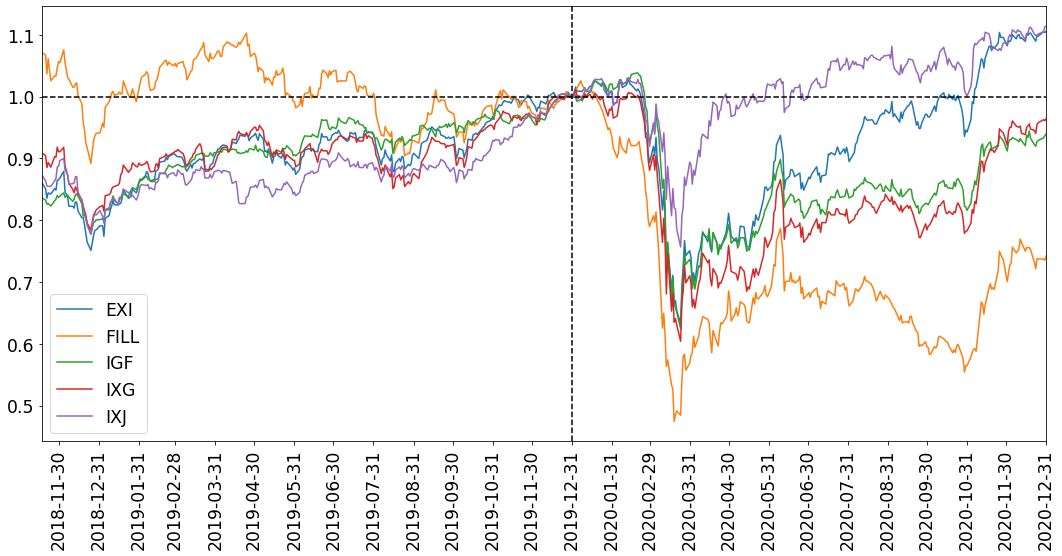
\includegraphics[width=1.15\textwidth]{bilder/Equity_ETP_1USD_Return_1.png}
        \caption{Equity ETPs' returns on a 1 U.S. dollar investment from end 2019 until end 2020}
        \label{fig:equity_etp_1usd_return_1}
    \end{figure}
    
    In figure \ref{fig:equity_etp_1usd_return_2}, we observe the great run and out-performance of the iShares Global Tech ETF with ticker IXN.
    
    % Data
    \begin{figure}[h!]
        \centering
        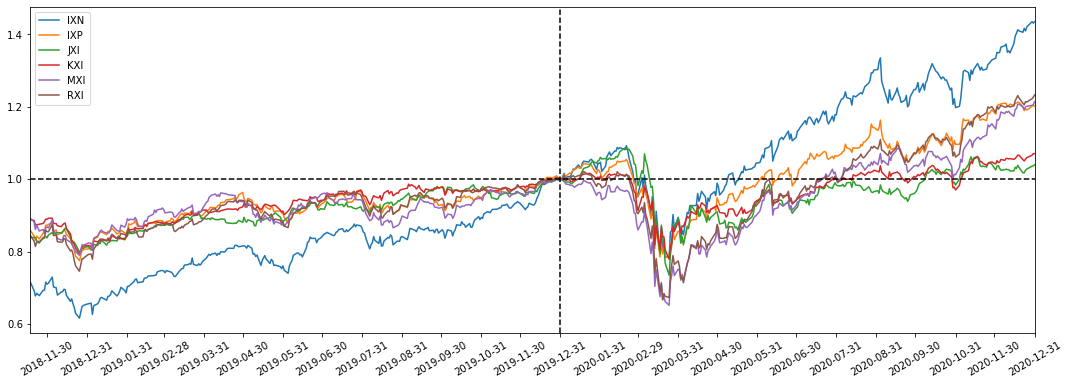
\includegraphics[width=1.15\textwidth]{bilder/Equity_ETP_1USD_Return_2.png}
        \caption{Equity ETPs' returns on a 1 U.S. dollar investment from end 2019 until end 2020}
        \label{fig:equity_etp_1usd_return_2}
    \end{figure}
    
    In figure \ref{fig:re_etp_1usd_return}, we can see the end-of-day absolute return on an investment of 1 U.S. dollar in the ETP selected as a proxy to represent the real estate asset class.
    
    %Data
    \begin{figure}[h!]
        \centering
        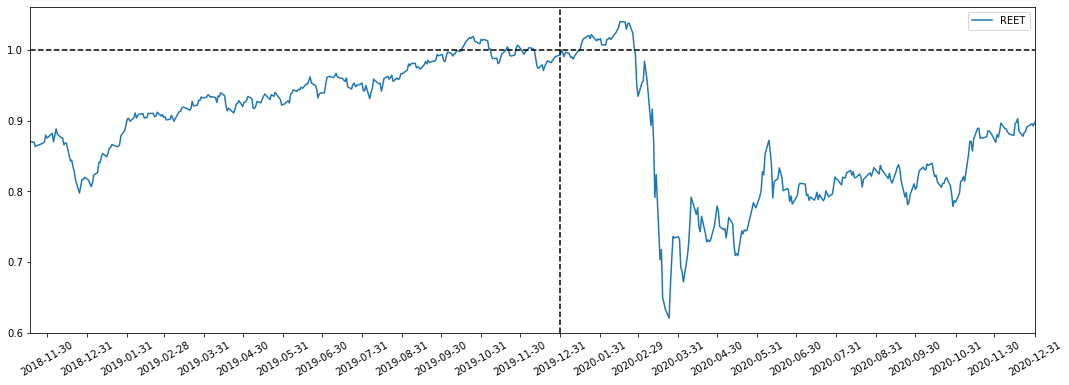
\includegraphics[width=1.15\textwidth]{bilder/RE_ETP_1USD_Return.png}
        \caption{Real Estate ETP returns on a 1 U.S. dollar investment from end 2019 until end 2020}
        \label{fig:re_etp_1usd_return}
    \end{figure}
    
    In figure \ref{fig:fi_etp_1usd_return}, we can see the end-of-day absolute return on an investment of 1 U.S. dollar in each of the selected fixed income ETPs from end 2019 until end 2020. The zero return level and the start of the backtesting period are marked by a horizontal and a vertical black dashed line respectively. The plot to the left of the vertical black dashed line represents the performances in the period used to warm-up the algorithm with data to be able to compute the first portfolio at the beginning of January 2020. The steep drop in both charts around March 2020 marks the results of the COVID-19 crisis, from which all fixed income ETFs recovered quickier than equity ETFs.
    
    % Data
    \begin{figure}[h!]
        \centering
        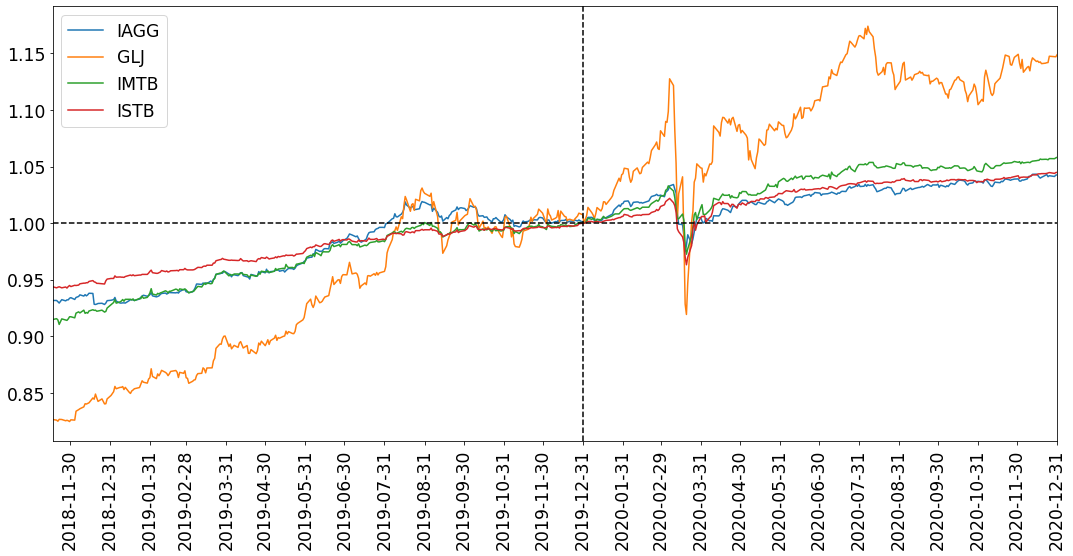
\includegraphics[width=1.15\textwidth]{bilder/FI_ETP_1USD_Return.png}
        \caption{Fixed Income ETPs' returns on a 1 U.S. dollar investment from end 2019 until end 2020}
        \label{fig:fi_etp_1usd_return}
    \end{figure}
    
    In figure \ref{fig:commodity_etp_1usd_return}, we can see the end-of-day absolute return on an investment of 1 U.S. dollar in each of the selected commodity ETPs from end 2019 until end 2020. The zero return level and the start of the backtesting period are marked by a horizontal and a vertical black dashed line respectively. The plot to the left of the vertical black dashed line represents the performances in the period used to warm-up the algorithm with data to be able to compute the first portfolio at the beginning of January 2020. The steep drop in both charts around March 2020 marks the results of the COVID-19 crisis. The red line represents the returns of the precious metals fund, which recovered quicker than the energy fund in green.
    
    % Data
    \begin{figure}[h!]
        \centering
        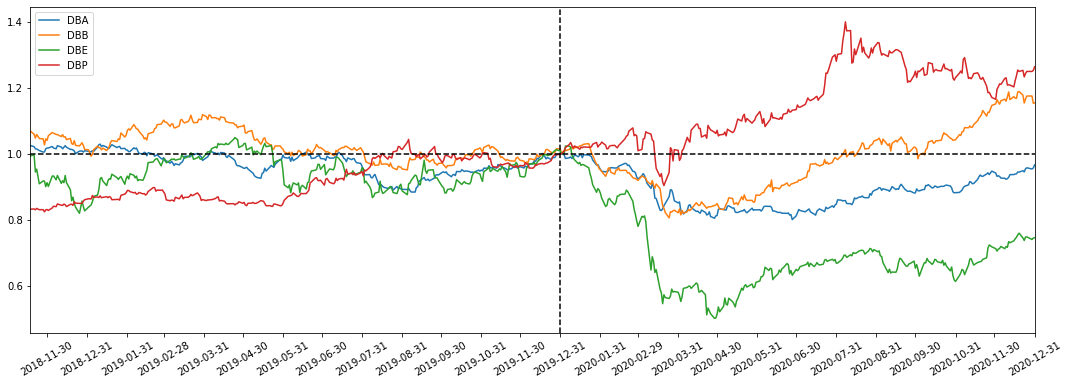
\includegraphics[width=1.15\textwidth]{bilder/Commodity_ETP_1USD_Return.png}
        \caption{Commodity ETPs' returns on a 1 U.S. dollar investment from end 2019 until end 2020}
        \label{fig:commodity_etp_1usd_return}
    \end{figure}

\subsection{Backtest Settings}\label{backtestsettingssec}
    In total, 12 portfolios are computed, corresponding to a backtesting period from January 1, 2020 to December 31, 2020 and monthly rebalancing-interval. The rebalancing occurs on the first trading day of each month at 10:00 AM New York time. An initial account balance of 10 million U.S. dollars is assumed, and margin calls are deactivated in order to better simulate the theoretical portfolios computed.
    
    For the computation of portfolio weights, the daily returns of the past 60 days is used as input. This last setting does not affect the equal weight portfolio construction method, because this naive method does not use any past data as input. The reason why we use 60 days of past data is because we need at least 20 periods of data to fulfil a necessary condition for the invertibility of the sample covariance matrix, and 60 days corresponds to 3 full trading months of data.
    
    
    
    In our practical implementation framework, we have selected $N = 20$ assets, therefore $T \geq 20$ must hold. This does however not guarantee that the covariance matrix has full rank and hence is invertible, because the condition $N \leq T$ is not a sufficient condition for that.
	
	There is not a single true underlying covariance matrix, but rather one that changes over time according to human behaviour and psychology, else every investor could compute optimal portfolios that would remain optimal over time. Therefore, it is worth to mention the trade-off between higher values of $T$, which lead to a more stable, with higher probability non-singular sample covariance matrix over time but at the same time make the portfolio optimisation less sensitive to changes in market trends and regimes, and lower values of $T$, which make the covariance matrix estimation process more sensitive to changes in market trends and regimes but make the portfolio optimisation process less stable. The asset manager should always take this into account, in order to reduce noise in the estimation while still using input parameters that allow to react to changes in the market. In the case of our practical implementation framework, we could, of course, have chosen a different value of $T$, and there is no mathematical reason to prefer $T=60$ to $T=59$ or $T=100$, for example. However, optimising the covariance matrix estimation process with respect to the number of observations used for its computation is not part of this work, and a 3-month past-data-window seems acceptable for the estimation of portfolios with a holding period of one month (optimal portfolios are computed and rebalanced each month).

\subsection{Portfolio Analyses}
    
    % Tools to analyse PFs: HHI for concentration, risk-adjusted returns, stability: turn-over volume, what else?
    
    The portfolios generated by each optimisation method in backtesting will be analysed with respect to risk-adjusted return, concentration and stability. The Sharpe ratio is the chosen measure to quantify risk-returns. To assess concentration, we will use a normalised version of the Herfindahl-Hirsch-Index (HHI). The normalisation step is necessary, because we will allow for short positions in our portfolios, and the HHI is only defined for positive portfolio weights. We will measure stability via the turnover of the portfolio.
    
    \begin{definition}[Sharpe Ratio \cite{franzen}] % Page 216
        Let $\mu_P \in \mathbb{R}$ be the return of the portfolio $P$ over a given period of time and $\sigma_P \in \mathbb{R}_{\geq 0}$ its standard deviation over that same period of time. Moreover, let $R_f \in \mathbb{R}$ be the risk-free rate of that given period. Then the \textbf{Sharpe Ratio of portfolio $P$ over the given period} $SR_P \in \mathbb{R}$ is given by
        \begin{align*}
            SR_P := \frac{\mu_P - R_f}{\sigma_P}
        \end{align*}
    \end{definition}
    
    \begin{remark}
        We do not compute the Sharpe ratio of the backtest separately, and rely upon QuantConnect's internal overall portfolio statistics for its computation, i.e. all Sharpe ratios presented here are the Sharpe ratios that appear in QuantConnect's backtesting results. QuantConnect computes the Sharpe ratio using the same definition as above, but using the annualised return of the portfolio in the backtest \cite{qcsharperatiocode}.
    \end{remark}
    
    % https://quant.stackexchange.com/questions/65525/herfindahl-hirsch-index-for-fx-portfolios?noredirect=1#comment92677_65525
    %To assess concentration, we choose Yager's entropy, because, in contrast to the Herfindahl-Hirsch-Index, Yager's entropy allows asset weights to be negative. 
    
    %\begin{definition}[Yager's Entropy \cite{yagerentropy}]
    %    Consider a portfolio with $n$ assets. Let $w_1, \dots, w_n \in \mathbb{R}$ be the weights associated to each of the $n$ assets in the portfolio. Then Yager's entropy $Q(w_1, \dots, w_n)$ is defined as
    %    \begin{align*}
    %        Q(w_1, \dots, w_n) := - \left( \sum_{i=1}^n \left| w_i - \frac{1}{n} \right|^z \right)^{\frac{1}{z}}
    %    \end{align*}
    %    where $z \in \mathbb{N}_{\geq 1}$ is a constant. \todo{change source to \url{https://www.sciencedirect.com/science/article/abs/pii/002002559400030F}}
    %\end{definition}
    
    %\begin{remark}
    %    \todo{add remark, that min entropy if equal weighted portfolio}
    %\end{remark}
    
    \begin{definition}[Herfindahl-Hirsch-Index \cite{chammas}] % Page 71 (85 of the PDF)
        Let $P$ be a portfolio containing $N$ assets with weights $w_i \in \mathbb{R}_{\geq 0}$ for all $i=1, \dots, N$, such that $\sum_{i=1}^N w_i = 1$. We define the \textbf{Herfindahl-Hirsch-Index (HHI)} as
        \begin{align*}
            HHI_P := \sum_{i=1}^N w_i^2
        \end{align*}
        For the general case of a portfolio $P$ with weights $w_i \in \mathbb{R}$ for all $i = 1, \dots, N$, we define the \textbf{normalised Herfindahl-Hirsch-Index (nHHI)} as
        \begin{align*}
            nHHI_P := \sum_{i=1}^N \left( \frac{|w_i|}{\sum_{j=1}^N |w_j|}\right)^2
        \end{align*}
        Obviously, $nHHI_P \leq HHI_P$ for the general case of a portfolio $P$ with weights $w_i \in \mathbb{R}$ for all $i = 1, \dots, N$.
    \end{definition}
    
    \begin{definition}[Turnover \cite{equalweight}]
        Consider a portfolio $P$ with $N$ assets. Let $w_{j,t+1} \in \mathbb{R}$ be the portfolio weight assigned to asset $i$ at time $t$ by the portfolio optimisation method, and let $w_{j,t^+} \in \mathbb{R}$ be the portfolio weight of asset $i$ before rebalancing at time $t+1$ for $i=1, \dots, N$ and $t=0, \dots, T$. The turnover of the portfolio $P$ is defined as
        \begin{align*}
            TO_P := \frac{1}{T} \sum_{t=0}^T \sum_{i=1}^N \left( \left| w_{i, t+1} - w_{i, t^+} \right| \right)
        \end{align*}
        where $T \in \mathbb{N}$ is the number of rebalancing points of the portfolio.
    \end{definition}
    
    This turnover quantity can be interpreted as the average percentage of wealth traded at each rebalancing point.
    
\subsection{Benchmark Portfolio Construction Methods}
    We use 2 naive portfolio allocation models, equal weight and inverse variance allocation, as benchmarks for the other 3 methods (Markowitz minimum volatility portfolio, Markowitz minimum volatility portfolio with covariance matrix shrinking and hierarchical risk parity) to estimate if the the increased complexity of the latter can be justified in form of better risk-adjusted returns, concentration and stability.